\documentclass[10pt,twoside,slovak,a4paper]{article}

\usepackage[slovak]{babel}
\usepackage[T1]{fontenc}
\usepackage[utf8]{inputenc}
\usepackage{graphicx}
\usepackage{booktabs}
\usepackage{url} % príkaz \url na formátovanie URL
\usepackage{hyperref} % odkazy v texte budú aktívne (pri niektorých triedach dokumentov spôsobuje posun textu)

\usepackage{cite}
\usepackage{natbib}
\usepackage{times}
\usepackage[dvips,dvipdfm,a4paper,centering,textwidth=14cm,top=4.6cm,headsep=.6cm,footnotesep=1cm,footskip=0.6cm,bottom=3.8cm]{geometry}

\pagestyle{headings}

\title{Nanoboty v medicíne}

\author{Jaroslav Sumbal, Andrej Švec\\[2pt]
	{\small Slovenská technická univerzita v Bratislave}\\
	{\small Fakulta informatiky a informačných technológií}\\
	{\small \texttt{sumbal13@fiit.stuba.sk, svec13@fiit.stuba.sk}}\\
	{\small Hlavný zdroj: \cite{Zdroj}}
	}

\date{\small 21. február 2015} % upravte



\begin{document}

\maketitle


\begin{abstract}


\end{abstract}

\section{Problémové prostredie}

Problémove prostredie je ľuďské telo. Je totiž veľmi zratiteľné. Stačí malý pád a zlomenina je na svete. Našťastie, väčšinu týchto fyzických zranení vieme napraviť, alebo si telo pomôže samo. Toto neplatí pre prípad zákernej choroby, akou je rakovina. Čo je to rakovina? Rakovina vznikne vtedy, keď sa niektoré bunky začnú chorobne množiť a brániť zdravým bunkám vykonávať svoju prácu. V dnešnej dobe existuje viacero druhov liečenia rakoviny, ale nefungujú dokonale. Nedajú sa vyliečiť všetky druhy rakoviny a niekedy sa dá len spomaliť ich priebeh. Preto je potrebné nové riešenie, ktoré ponúka pole nanotechnológii.
\\
Ľuďské telo je veľmi komplikované a preto treba veľmi inteligetné riešenie. Je potrebné rozoznať zdravé bunky od tých chorých, aby sa pacientovi náhodou neprihoršilo. Ďalšia nevyhnutnosť je dobrý transportný systém. Telo už taký má, je to krvný obeh. Avšak krvný obeh ponúka plejádu možností, veľa rôznych ciest. Ktorou sa vydať? Táto otázka potrebuje premyslenú odpoveď, aby bola liečba čo najefektívnejšia.
\\
Veľký problém taktiež predstavuje imunitný systém ľuďského tela. Ako presvedčiť telo, že nanoboty sú preň dobré aby ich nezničil? Nie je to vôbec ľahké, keď si uvedomíme, že niekedy je aj transplantovaný orgán odvrhnutý, teda niečo prirodzené telu. A tu je treba aby prijalo niečo syntetické. Je to jeden zo základných problémov, ktorý treba vyriešiť, aby vôbec celý tento výskum mal zmysel.

\section{Opis znalostného konateľa}

\subsection{Ciele}
Nanoboty sú vpustené do organizmu za účelom ozdravenia organizmu a to odstránením rakovinotvorných buniek, prítomných v organizme. Takisto je cieľom, aby bolo minimalizované množstvo zdravých buniek, ktoré boli zničené pri odstraňovaní rakovinotvorných buniek. Teda je dôležité aby pri odstraňovaní chorých buniek neboli poškodené a znižené aj zdravé bunky. Nakoniec ide aj o minimalizáciu času potrebného na nájdenie rakovinotvornej bunky od doby jej vzniku.

\subsection{Vnemy}
Vstupmi pre nanobota sú rôzne chemické látky, ktoré nájde v bunkách a ich koncentrácia, tvar bunky, sekvencia DNA, ktorú vie prečítať. Keďže nanobot musí vedieť komunikovať s ostatnými nanobotmi, tak je pre neho vstupom aj ľubovoľná informácia od ostatných nanobotov. Ide najmä o informácie o sekvenciách DNA a o koncentrácii rôznych chemických látok v krvi.

\subsection{Akcie}
Nanobot musí na základe vnemov vedieť reagovať, a to buď zničením, alebo ponechaním bunky. Najdôležitejším faktorom je pri tomto procese, správne rozlíšenie zdravej bunky od chorej bunky. Pri tomto je nutné použiť rôzne analýzy, ďalej opísané v časti \ref{sec:spravanie}. Pri týchto analýzach je nutné, aby nanobot vedel komunikovať ostatným nanobotom informácie.


\section{Znalosti konateľa}
\label{sec:znalosti}
Rakovinotvorné bunky majú oveľa väčšiu spotrebu cukru. Takisto je možné tieto bunky detekovať na základe toho, že majú poškodenú DNA. Nanobot môže vyhľadať a prečítať DNA v bunkovom jadre a na základe toho vyhodnotiť, či je bunka chorá, alebo nie.
\cite{Wikipedia-nador,cancer-cell-metabolism}

\section{Správania konateľa}
\label{sec:spravanie}
Nanobot musí byť schopný analyzovať prostredie na základe správania sa rakovinových buniek. Ako bolo opísané v časti \ref{sec:znalosti} rakovinové bunky majú vyššiu spotrebu cukru a takisto majú poškodenú DNA. Správanie nanobotov teda vychádza z týchto dvoch predpokladov.
\\
Množstvo cukru, ktoré normálne bunky spotrebujú kolíše v závislosti od jedinca a jeho fyzickej a psychickej aktivity, typu bunky a ďalších iných faktorov. V prípade zvýšenej fyzickej aktivity rastie aj konzumácia cukru. Cukor konzumujú najmä mozgové bunky, červené krvinky, alebo svalové bunky. Tieto faktory sú teda problematické pri určovaní, či je bunka rakovinová, alebo nie je.
\\
Ďalším problémom je zistenie pravej, teda nepoškodenej, sekvencie DNA. Bunky majú zapísanú DNA sekvenciu v jadre. Náš nanobot sa teda musí vedieť dostať do jadra a prečítať sekvenciu DNA. Avšak táto sekvencia môže byť poškodená, čo môže nastať mutáciou génov. K mutáciám dochádza najmä pri prepisovaní sekvencií DNA.
\cite{Wikipedia-glukoza, Wikipedia-jadro, Wikipedia-mutations}

Všetky tieto problémy vedú k tomu, že nanoboty musia byť schopné komunikácie medzi sebou. Nanoboty môžu získať dobrý obraz o tom, ktorá sekvencia DNA je správna až po analyzovaní veľkého množstva buniek, pretože až potom bude pravdepodobnosť chyby menšia. Takisto je potrebné zmapovať množstvo cukru, ktoré bunky spotrebujú, aby sme boli schopní určiť, ktoré bunky majú nadmernú spotrebu cukru. Teda po nasadení nanobotov do prostredia je nutné vyčkať nejaký čas na analýzu prostredia. Výstupom z tejto fázy sú dve hodnoty: hraničná hodnota pre konzumáciu cukru v krvi a hraničná hodnota pre chybovosť v sekvenciách DNA. Po analýze prostredia nanoboty začnú odstraňovať rakovinové bunky, teda bunky, ktorých spotreba cukru presahuje určenú hraničnú hodnotu a ktorých DNA prekračuje hraničnú chybovosť. Jednotlivé fázy sú znázornené aj v obrázku \ref{f:spravanie}.

\begin{figure}[tbh]
\label{f:spravanie}
\centering1
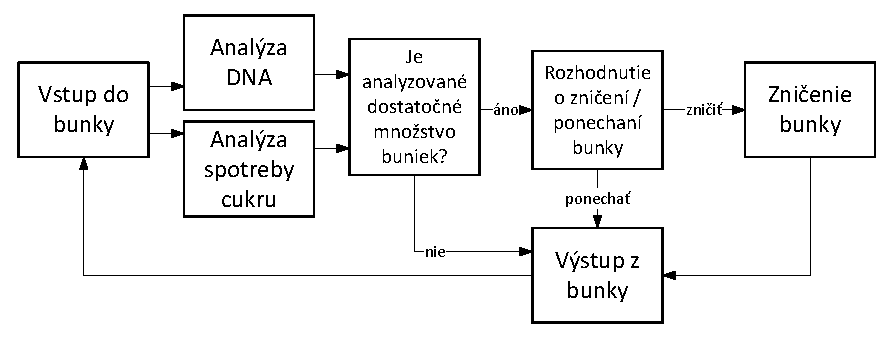
\includegraphics[scale=0.9]{spravanie.pdf}
\caption{Správanie nanobota v organizme}
\end{figure}

\section{Záver}

\listoffigures
\bibliography{zdroje}
\bibliographystyle{unsrt}
\end{document}

